\begin{frame}{Our challenge and philosophy}
\key{Challenge}\par
Full-image reconstruction rewards a model for remembering the digit and the decoration around it. Both can reduce pixel error. Only the digit defines the desired group.
\par\bigskip
\key{Philosophy}\par
Change the background while holding the handwriting fixed. Use what persists across paired views as the reconstruction target, then measure whether the digit keeps its cluster.
\notefoot{A known stripe direction supplied our first test. Detached geometric marks let us vary the background while preserving every stroke pixel.}
\end{frame}

\begin{frame}{A background change that leaves every stroke intact}
\centering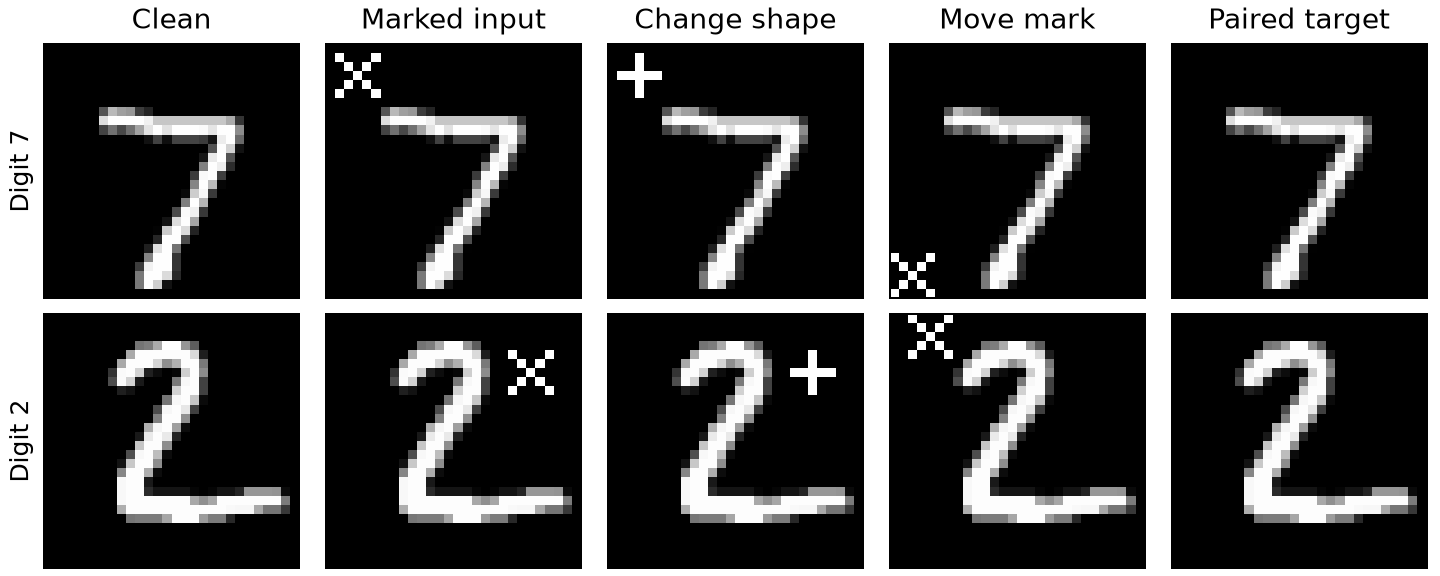
\includegraphics[width=.9\linewidth,height=.62\textheight,keepaspectratio]{../figures/geometry.png}
\notefoot{Both symbols use nine pixels. Every placement leaves a one-pixel gap from the ink. The paired target keeps values shared by the marked input and the moved view.}
\end{frame}

\begin{frame}{Four ways to train the autoencoder}
\begin{tabular}{@{}lp{.65\linewidth}@{}}
\toprule
Pretraining & What the decoder is rewarded for\\ \midrule
Fixed input & Reproducing the digit and its original mark.\\[3pt]
Augmentation & Reproducing whichever shape and site appear that epoch.\\[3pt]
Paired target & Reproducing pixels shared by two views with the mark at different sites.\\[3pt]
Gaussian prior & Reproducing the current view, with higher weight near the image center.\\
\bottomrule
\end{tabular}
\notefoot{The last three arms see the same augmented inputs. All four use the same initialization seed, training budget and ordinary IDEC fine-tuning.}
\end{frame}

\begin{frame}{What changes when the background mark moves?}
\key{Reconstruction after pretraining}\par
Show the frozen autoencoder the same digit twice. Project the change in its reconstructed image onto the actual movement of the mark. A score of one reproduces the full displacement. A score of zero has no component along it.
\par\bigskip
\key{Assignments after clustering}\par
Hold the model fixed. Move the mark or change its shape, and count how often the digit switches clusters. Score digit accuracy separately, using the label mapping fitted on training digits after optimization.
\notefoot{12,000 training and 10,000 held-out digits. The decoder check is an exploratory pretraining replay. Each test digit serves as its own control.}
\end{frame}

\begin{frame}{Clustering stability and digit accuracy}
\centering\scriptsize\begin{tabular}{lrrrrr}
\toprule
Pretraining & Marked ACC & Clean ACC & Move flips & Shape flips & Decoder response\\
\midrule
Full, fixed input & 67.15 & 69.84 & 6.20 & 5.35 & 0.00585\\
Augmentation only & 71.02 & 72.96 & 4.34 & 3.43 & 0.00313\\
Aug. + paired target & 71.55 & 73.02 & 4.18 & 3.59 & 0.00085\\
Aug. + Gaussian & 72.91 & 74.34 & 4.16 & 3.37 & 0.00278\\
\bottomrule
\end{tabular}

\par\medskip\normalsizeAugmentation cut movement flips from 6.20\% to 4.34\%, with a reduction in every seed. The paired target further suppressed the decoder's already weak mark response. Gaussian weighting gave the highest mean marked ACC (72.91\%).

\notefoot{Means across five seeds and 10,000 held-out digits. ACC and flip rates in percent. Decoder response measures reconstruction of the mark's displacement after pretraining; a perfect response is one.}
\end{frame}
